\section{Results}
    \subsection{Summary}
        We found 43 publications describing the development or adaption of \gls{ohd-gan}, presented in Table \ref{tab:3:publications}. We can generalize the data addressed in each of these publications into one of two categories: time-dependent observations, such as time-series, or static representation in the form of feature vectors such as tabular rows. We briefly bring attention to the lack of multi-relational tabular representations, the primary form of \gls{ehr}, and further discuss the subject in latter sections.\par
        
        Most efforts propose adaptations of current algorithms to the characteristics and complexities of \gls{ohd}. These include multi-modality of marginal distributions or non-Gaussian real-valued features, heterogeneity, a combination of discrete and real-valued features, longitudinal irregularity, complex conditional distributions, missingness or sparsity, class imbalance of categorical features and noise.\par 
        
        While these properties may make training a useful model difficult, the variety of applications that are highly relevant and needed in the healthcare domain provides sufficient incentive. The most cited motives are, as one would expect, to cope with the often limited number of samples in medical datasets and to overcome the highly restricted access to \gls{ohd}. The potential of releasing privacy-preserving \gls{sd} freely is a common subject. Publications considering privacy evaluate the effect on utility of applying \gls{dp} to their algorithm, propose alternatives privacy concepts and metrics, or only concentrate on the subject of privacy.\par
        
    \subsection{Motives for developing OHD-GAN}
        Some claim that the ability to generate synthetic is becoming an essential skill in data science \cite{Sarkar2018}, but what purpose can it serve in the medical domain? The authors mention a wide range of potential applications. We briefly describe the four prevailing themes in the following sections: data augmentation (Sec.\ref{sec:augmentation}), privacy and accessibility (Sec.\ref{sec:access_privacy}), precision medicine (Sec.\ref{sec:precision_med}) and  modelling simulations (Sec.\ref{sec:models_twins}). 

        \subsubsection{Data augmentation}\label{sec:augmentation}
    
            Data augmentation \todo{define} is mentioned in nearly all publications. Although counter-intuitive, \gls{gan} can generate \gls{sd} that conveys more information about the real data distribution. Effectively, the real-valued space distribution of the generator produces a more comprehensive set of data points, valid, but not present in the discrete real data points. A combination of real and synthetic training data habitually leads to increased predictor performance \cite{Wang_2019,Che_2017,Yoon2018-ite, yoon2018imputation, Yang_2019_impute_ehr, Chen_2019, cui2019conan, Che_2017}. A more intelligible way to seize the concept from the point of view of image classification, known as invariances, perturbations such as rotation, shift, sheer and scale \cite{antoniou2017data}.\par 
            
            Similarly, domain translation \todo{define} and \gls{semi-sup} training approaches with \glspl{gan} could support predictive tasks that lack data with accurate labels, lack paired samples or suffer class imbalance \cite{Che_2017,mcdermott2018semi, Yoon2018-ite}. Another example is correcting discrepancies between datasets collected in different locations or under different conditions inducing bias \cite{Yoon2018-radial}. \glspl{gan} are also well adapted for data imputation, were  entries are \gls{mar} \cite{yoon2018imputation}. 

        \subsubsection{Enhancing privacy and increasing data accessibility}\label{sec:access_privacy}
    
            Most authors see \gls{sd} as the key to unlocking the unexploited value of \gls{ohd} hindering machine learning, and scientific progress \cite{Beaulieu-Jones2019-ct, baowaly_2019_IEEE,baowaly_2019_jamia,Che_2017,esteban2017real,Fisher2019,severo2019ward2icu} or education \cite{laderas_teaching_2018}. We can broadly describe preserving privacy as reducing the risk of \gls{re-iden} to an acceptable level. It quantifies this level of risk when releasing data anonymized with \gls{dp}.\par
    
            Due to its artificial nature, \gls{sd} is put forward to forgo the tight restrictions on data sharing, while potentially providing greater privacy guarantees \cite{Beaulieu-Jones2019-ct, baowaly_2019_IEEE, baowaly_2019_jamia,esteban2017real,Fisher2019,walsh2020generating, chin2019generation}. Enabling access to greater variety, quality and quantity of \gls{ohd} could have positive effects in a wide range of fields, such as software development, education, and training of medical professionals. The fact remains that \glspl{gan} do not eliminate the risk of reidentification. Considering none of the synthetic data points represent actual people, the significance of such an occurrence is unclear. It is possible to combine both methods, and \gls{gan} training according to \gls{dp} shows evidence of reducing the loss of utility compared to \gls{dp} alone.
    
        \subsubsection{Enabling precision medicine}\label{sec:precision_med}
    
            The application to precision medicine involves predicting outcomes conditioned on a patient's current state and history. Simulated trajectories could help inform clinical decision making by quantifying disease progression and outcomes and have a transformative effect on healthcare \cite{walsh2020generating, Fisher2019}. Ensembles of stochastic simulations of individual patient profiles such as those produced by \gls{crmb} could help quantify risk at an unprecedented level of granularity \cite{Fisher2019}.\par
            Predicting patient-specific responses to drugs is still a new field of research, a problem known as \gls{ite}. Estimating \glspl{ite} is persistently hampered by the lack of paired counterfactual samples \cite{Yoon2018-ite, chu2019treatment}. To solve similar problems n medical imaging, various \gls{gan} algorithms were developed for domain translation, mapping a sample from its to original class to the paired equivalent. This includes bidirectional transformations, allowing \gls{gan} to learn mappings from very few, or a lack of paired samples \cite{Wolterink2017DeepMT, CycleGAN2017, mcdermott2018semi}.
    
        \subsubsection{From patient and disease models to digital twins}\label{sec:models_twins}
    
            A well-trained model approximates the process that generated the real data points. The relations learned by the model, its parameters, contain meaningful information if we can learn to harness it. Data-driven algorithms evolve as our understanding of their behavior improves. We incorporate new concepts in the algorithms leading to further understanding, iterativly blurring the line with theory-driven approaches \cite{Hand2019}. Interpretability is a growing field of research concerned with understanding how the learned parameters of a model relate. In other words analysing the representation the algorithm has converged to and deriving meaning from obscure logic. Incorporating new understanding in the architecture of algorithms shift the view from a data-driven to a theory-driven perspective \cite{Hand2019}. As we purposefully build structure in our algorithms from new understanding, we may get the chance to explore meaningful representations that would otherwise be beyond our reasoning.\par 
            
            Approaching these ideas from above, the concept of "digital twins" represents in a way the ultimate realization of \gls{pm}. A common practice in industrial sectors is high-fidelity virtual representations of physical assets. Long-term simulations, that provide an overview and comprehensive understanding of the workings, behavior and life-cycle of their real counterparts. The state of the models is continuously updated from theoretical data, real data, and streaming \gls{iot} indicators.\par
            Intently conditioned input data allows the exploration of specific events or conditions. In a position paper on the subject, Angulo et al. draw the parallels of this technique with the current needs in healthcare and the emergence of the technologies for actionable models of patients. \cite{angulo2019towards,Angulo_2020}. The authors bring up the rapid adoption of wearables that are continuously monitoring people's physiological state.\par 
            
            Wearables are one of many mobile digitally connected devices that collect patient data over a broad range of physiological characteristic and behavioral patterns \cite{coravos2019developing}. This emerging trend known as \gls{dbio} has already led to studies demonstrating predictive models with the potential for improved patient care \cite{snyder2018best}. Through continuous lifelong learning, integrating  multiple modes of personal data, generative patient models could inform diagnostics of medical professionals and also enable testing treatment options. In their proposal, \gls{gan} are an essential component of the ecosystem to ensure patient privacy and to provide bootstrap data. Fisher et al. already use the term "digital twin" to describe their process, noting that they present no privacy risk and enable simulating patient cohorts of any size and characteristics \cite{walsh2020generating}.
        
            
\newcolumntype{R}{>{\raggedright\arraybackslash}p{0.20\textwidth}}
\newcolumntype{M}{>{\raggedright\arraybackslash}p{0.40\textwidth}}
\newcolumntype{N}{>{\raggedright\arraybackslash}p{0.30\textwidth}}
\newcommand{\specialcell}[2][c]{%
  \begin{tabular}[#1]{@{}l@{}}#2\end{tabular}}
  
\begin{center}
    
    \setlength\LTleft{0pt}
    \setlength\LTright{0pt}
    \scriptsize
    \setlength{\extrarowheight}{1em}
    
    \begin{longtable}[l]{@{}p{0.10\textwidth}NMR@{}} 
        \kill
        \caption{Summary of the publication included in the review.\label{tab:3:publications}}\\
        \hline
        Publication & Algorithm(s) & Focus, algorithms and techniques & Data type \\ 
        \hline
        \endfirsthead
        \caption[]{Summary of the publication included in the review (Continued).}\\
        \hline
        Publication & Algorithm(s) & Focus, algorithms and techniques & Data \\ 
        \hline
        \endhead
        \hline 
        \endfoot
        
        \quad 2017 & & & \\
        \hline
        \citeauthor{Choi2017-nt} & \gls{medgan} 
        & Incompatibility of back-propagation with discrete features. \gls{ae}, \gls{mb-avg}, \gls{bn}, \gls{sc}, \gls{ad}, \gls{pda}.
        & Binary occurences or counts of medical codes.\\
        
        \citeauthor{yahi2017generative} & \gls{medgan} adaptation
        & \Gls{dle} on continuous time-series, multi-modality. \gls{t-sne}.
        & Paired pre/post treatment exposure time-series\\
        
        \citeauthor{esteban2017real} & \gls{rgan}, \gls{rcgan} 
        &  Adversarial training of (conditional) \glspl{rnn} on time-series, evaluation, privacy. \gls{lstm}, \gls{cgan}, \gls{dp-sgd}.
        & Regularly observed \gls{rvts}\\
        
        \citeauthor{Xiao2017-lh} & \gls{wgantpp} 
        & Temporal Point Processes. \gls{lstm}, \gls{wgan}, Poisson process.
        & Sporadic occurrences, hospital visits.\\
        
        \citeauthor{Che_2017} & \gls{ehrgan}, \gls{ssl-gan} 
        & Semi-supervised augmentation, transitional distribution. 1D-CNN, Word2vec, \gls{vcd}.
        & \Gls{dts}, sequences of medical codes. \\
        
        \citeauthor{dash2019synthetic} & \gls{healthgan} & Sleep patterns, stratification by covariates. & Binary over multiple visits.\\
        
        \hline
        \quad 2018 & & & \\
        \hline
        
        \citeauthor{Camino2018-re} & \raggedright \gls{mc-arae}, \gls{mc-medgan}, \gls{mc-gumbelgan}, \gls{mc-wgan-gp}
        & Improving training process. \gls{medgan}, \gls{wgan-gp}, \gls{gumbel-gan}, \gls{arae}.
        & Multiple categorical variables. \\
        
        \citeauthor{mcdermott2018semi} & \gls{cwr-gan}
        & Cycle-consistent semi-supervised regression learning, unpaired data, class imbalance. \gls{wgan} \gls{cycle-gan} \gls{ite}
        & ICU \gls{rvts}, lack of paired samples, \gls{sd}. \\
        
        \citeauthor{Yoon2018-ite} & \gls{ganite} 
        & \gls{ite}, unobserved counterfactual, multi-label classification, uncertainty. \gls{cgan} pair.
        & Feature, treatment and outcome vectors.\\
        
        \citeauthor{Yoon2018-radial} & \gls{radialgan} 
        & Multi-domain translation, features and distribution mismatch, cycle-consistency, augmentation. \gls{cgan}, \gls{wgan}.
        & Tabular, discrete and continuous.\\
        
        \citeauthor{yoon2018imputation} & \gls{gain}
        & Tabular data imputation. \gls{mcar}, \gls{cgan}.
        & Real-valued, tabular with entries \gls{mcar}.\\
        
        \hline
        \quad 2019 & & & \\
        \hline
        
        \citeauthor{Wang_2019} & \gls{sc-gan}
        & Capturing mutual influence in time-series. Coupled generator pair. Treatment recommendation task. \gls{lstm}, \gls{cgan}.
        & \Gls{rvts} of patient state and medication dosage data.\\
        
        \citeauthor{baowaly_2019_IEEE} & \gls{medbgan}
        & Improving training process. \gls{medgan}, \gls{bgan}.
        & Binary occurences or counts of medical codes.\\
        
        \citeauthor{baowaly_2019_jamia} & \gls{medbgan}, \gls{medwgan}
        & Improving training process. \gls{medgan}, \gls{bgan}, \gls{wgan}.
        & Binary occurences or counts of medical codes.\\
        
        \citeauthor{severo2019ward2icu} & \gls{cwgan-gp} 
        & Generation and public release of dataset. Protecting commercial sensitive information. Class imbalance. \gls{cwgan-gp}, \gls{cgan}.
        & Physiological \gls{rvts}.\\
        
        \citeauthor{chin2019generation} & \gls{wgan}
        & Heterogeneous mixture of dense and sparse features. Privacy and evaluating the introduction of bias. \gls{wgan}, \gls{wgan-gp}, \gls{msn}, \gls{dp} aware optimizer from Tensor-flow. \citeauthor{tensorflow-privacy}.
        & Binary, real-valued and categorical.\\
        
        \citeauthor{Jordon2019} & \gls{pate-gan}
        & Alternative differential privacy, adaptation of the  \gls{pate} framework.
        & Demographic and binary.\\
        
        \citeauthor{torfi2019generating} & \gls{corgan}
        & \gls{cnn} architecture, capturing feature correlations, evaluating realism, privacy evaluation using \gls{mi}. 1D-\gls{cae}.
        & Binary occurences or counts of medical codes.\\
    
        \citeauthor{chu2019treatment} & \gls{adtep}
        & \gls{ite}, two independent \gls{ae} for patient and treatment feature sets, trained adversarially in combination, and outcome predictor from latent representation. &
         \Gls{ehr} data, not specified.\\
        
        \citeauthor{Jackson_2019} & \gls{medgan}
        & Evaluating medgan with the addition of demographics features.
        & Demographic features and binary occurences or counts of medical codes. \\
        
        \citeauthor{yu2019rare} & \gls{ssl-gan}
        & Rare disease detection, \gls{ssl}, leveraging unlabeled \gls{ehr} data, medical code embedding network.  \gls{lstm}.
        & Diagnosis and prescription codes.\\
        
        \citeauthor{Yang_2019_cdss} & \gls{cgan}
        & Class imbalance, low count of minority class. Semi-supervised learning combining \gls{st} and \gls{ct} with a \gls{cgan} for a \gls{iot} application.
        & Twenty medical datasets from the UCI repository, types unspecified.\\
        
        \citeauthor{Yang_2019_ehr} & \gls{gcgan}
        & Capturing the correlations between different categories of medical codes and the outcome.  \gls{corrnn}, \gls{t-gan}, \gls{t-wgan}.
        & Binary occurences or counts of medical codes.\\
        
        \citeauthor{Yang_2019_impute_ehr} & \gls{cgain}
        & Improve on \gls{gain} for categorical variable using fuzzy encoding of the features. 
        & Categorical (multi-class and multi-label) real-valued.\\
        
        \citeauthor{Camino2019} & \gls{gain}, \gls{gain}+\gls{vs}, \gls{vae}, \gls{vae}+\gls{it}, \gls{vae}+\gls{bp},  \gls{vae}+\gls{vs},  \gls{vae}+\gls{vs}+\gls{it}, \gls{vae}+\gls{vs}+\gls{bp}
        & Benchmark and improve on generative imputation with \gls{gain} and \gls{vae}. & Categorical and real-valued. Mostly not \gls{ohd}\\
        
        \citeauthor{Beaulieu-Jones2019-ct} & \gls{ac-gan} 
        & Evaluating if differentially private GANs that is valid reanalysis while ensuring privacy.  \gls{dp}, \gls{cgan}.
        & Physiological \gls{rvts}.\\
        
        \citeauthor{Xu2019-ay} & \gls{ctgan}
        & Non-Gaussian multi-modal distribution of continuous columns and imbalanced discrete column in tabular data. Evaluation benchmark.  \gls{cgan} \gls{tbs} \gls{msn} \gls{wgan-gp} \gls{gumbel-gan}
        & Tabular real-valued and categorical.\\
        
        \citeauthor{yale2019ESANN} & \gls{healthgan}
        & Privacy metrics and over-fitting.  \gls{mi}, \gls{nnaa}, \gls{pl}, \gls{dt}
        & Categorical demographics, real-valued and binary medical codes.\\
        
        \citeauthor{Fisher2019} & Adversarially trained \gls{crmb}
        & Simulation of patient trajectories from their baseline state, disease prediction and risk quantification, missingness.\gls{crmb}.
        &  Binary, ordinal, categorical, and continuous, 3 months intervals.\\
        
        \hline
        \quad 2020 & & & \\
        \hline
        
        \citeauthor{walsh2020generating} & Adversarially trained \gls{crmb}
        & Digital twins, disease prediction and risk quantification, missingness.   \gls{crmb}.
        & Binary, ordinal, categorical, and continuous, 3 months intervals.\\
        
        \citeauthor{Yale_2020} & \gls{healthgan}
        & Metrics to capture a synthetic dataset’s resemblance, privacy, utility and footprint. Evaluating applications. Application case studies, Reproducibility of studies with \gls{sd}.  \gls{nnaa}, \gls{pl}, \gls{do}, \gls{medgan}, \gls{wgan-gp}, \gls{sdv}, 
        & Real-valued and categorical. Demographics, vital signs, diagnoses, and procedures.\\
        
        \citeauthor{tanti2019} & \gls{dp-auto-gan}
        & Privacy, \gls{medgan} adaptation, evaluation metrics.  \gls{dp-sgd} \gls{ae} \gls{medgan} \gls{rdp}
        & Medical data: binary. Non-health data: categorical and real-valued.\\
        
        \citeauthor{BaeAnomiGAN2020} & \gls{anomigan}
        & Probabilistic scheme that ensures \textit{indistinguishability} of the \gls{sd}, than can be viewed as encrypted.  \gls{dp} \gls{cnn}
        & Binary occurences of medical codes.\\
        
        \citeauthor{cui2019conan} & \gls{conan}
        & Complementary \gls{gan} in a rare disease predictor model that generates positive samples from negatives to alleviate class imbalance.
        & Embedding vectors representing multiple patient visits and conditions.\\
        
        \citeauthor{zhu_2020} & \gls{glugan}
        & Adversarialy trained \gls{rnn} to predict the upcoming time-step in physiological time-series conditioned on the past observations.  \gls{rnn}, \gls{cnn}, \gls{gru}.
        & \Gls{rvts} of blood glucose measurements, discrete patient submitted features.\\
        
        \citeauthor{chen2019ganleaks} & \gls{medgan}, \gls{wgan-gp}, DC-GAN
        & Privacy analysis of generative models.   \gls{mi}, \gls{fullbba}, \gls{partbba}, \gls{wba}, \gls{dp-sgd}.
        & Binary vector of medical codes.\\
        
        \citeauthor{chincheong2020generation} & \gls{wgan-dp}
        & Heterogeneous data, effect of differential privacy on utility.   \gls{wgan} \gls{dp}
        & Categorical, continuous,  ordinal, and binary. Dense or sparse.\\
        
        \citeauthor{Camino2020bench} Initially a comparison \glspl{gan} and \glspl{vae}, but they choose instead to bring attention to the problem of benchmarking. Analysis of problematic,  requirements and suggestions. & Real-valued and categorical.
        
        \citeauthor{Zhang2020} & \gls{emr-wgan}
        & Improving training, evaluation metrics, sparsity.  \gls{wgan}, \gls{bn}, \gls{ln}, \gls{cgan}.
        & Binary occurences of medical codes. Low-prevalence of codes. \\
        
        \citeauthor{yan2020generating} & \gls{heterogan}
        & Improvements on \gls{emr-wgan} incorporating record-level constraints in the loss function.   \gls{wgan}, \gls{bn}, \gls{ln}, \gls{cgan}, \gls{mi}, \gls{pda}.
        & Binary, categorical and real-valued.\\
        
        \citeauthor{ozyigit2020generation} & \gls{rsdgm}
        & Exploring the feasibility of various methods to generate synthetic datasets.   \gls{wgan}
        & Real-valued and categorical.\\
        
        \citeauthor{Yoon2020-anon} & \gls{ads-gan}
        & Identifiability view of privacy. Generator conditioned on real samples inputs with an identifiability loss to satisfy the identifiability constraint.   \gls{wgan} \gls{wgan-gp} \gls{dp} alternative.
        & Real-valued and binary.\\
        
        \citeauthor{Goncalves2020} & \gls{mc-medgan}
        & Comparison of \glspl{gan} with statistical models to generate synthetic data, evaluation metrics.   \gls{mi}, \gls{ad}.
        & Categorical and real-valued.\\
           
        \hline
        
    \end{longtable}
\end{center}

    \subsection{Data Types and Feature Engineering}

        No publications made use of \gls{ohd} in its initial form, patient records in \gls{ehr} composed of many related tables (normalized form). The complexity of a model would explode when maintaining referential integrity and statistics between multiple tables. The hierarchy by witch these would interact with each other conditionally is no less complicated \cite{Buda2015, Patki_2016, Zhang2015, Tay2013}. There are published \gls{gan} algorithms made to consume normalized database in their original form. In all publications we considered, feature engineering was used to adapt the data to task requirements, or to promising algorithms that fit the data characteristics. They transform the data into one of four modalities: time series, point-processes, ordered sequences or aggregates described in Fig. \ref{tab:features}.

        \begin{table}[H]
        \footnotesize
        \caption{Types of observational health data and features engineering}\label{tab:features}
    
        \begin{tabularx}{\textwidth}{@{}p{0.15\textwidth}p{0.3\textwidth}p{0.3\textwidth}X@{}} \toprule
            Type & Values and structure & Challenges & Features engineering\\ \midrule
            
            \textbf{Time-series}\newline
            \textit{Continuous}\newline 
            \textit{Regular}\newline
            \textit{Sporadic}
            &\begin{minipage}[t]{0.3\textwidth}{
            \begin{itemize}[leftmargin=*]  
                \item Timestamped observations 
                \item Continuous, ordinal, categorical and/or multi-categorical
                \item Recorded continuously by medical devices, following a schedule by medical professional, or when necessary
            \end{itemize}}
            \end{minipage}
            &\begin{minipage}[t]{0.3\textwidth}{
            \begin{itemize}[leftmargin=*]  
                \item Observations are often \gls{mar} across time end dimensions, erroneous, or completely absent for certain patients.
                \item Time-series of different concepts are often highly correlated and their influence on one another must be accounted for.
             \end{itemize}}
             \end{minipage}
            & Imputation coupled with training \newline Regular \newline Data imputation \newline Binning in into fixed-size intervals \newline Combination of binning and imputation \\
            
            \textbf{Point-processes} 
            &\begin{minipage}[t]{0.3\textwidth}{
            \begin{itemize}[leftmargin=*]  
                \item Series of timestamped observations of one variable or medical concept per patient
            \end{itemize}}
            \end{minipage}
            &\begin{minipage}[t]{0.3\textwidth}{
            \begin{itemize}[leftmargin=*]  
                \item \todo{Intensity functions, paramtric models}
            \end{itemize}}
            \end{minipage}
            & Series of events reduced to the time interval between each consecutive occurrence. \\ 
            
            \textbf{Ordered \linebreak sequences} 
            & \begin{minipage}[t]{0.3\textwidth}{
            \begin{itemize}[leftmargin=*]  
                \item Ordered vectors representing one or more patients visits
                \item Medical codes associated with the diagnoses, procedures, measurements and interventions
            \end{itemize}}
            \end{minipage}
            & Variable length\newline High-dimensional\todo\newline Long-tail distribution of codes 
            & Sequences are projected into a trained embedding that preserves semantic meaning according to methods borrowed from NLP\\
            
            \textbf{Tabular}\newline Denormalized\newline Relational
            &\begin{minipage}[t]{0.3\textwidth}{
            \begin{itemize}[leftmargin=*]  
                \item Medical and demographic variables aggregated in tabular format
                \item Continuous, ordinal, categorical and/or multi-categorical features
            \end{itemize}}
            \end{minipage}
            & Medical history is aggregated into a fixed-size vector of binary or aggregated counts of occurrences and combined with demographic features.\\
            
            \bottomrule
        \end{tabularx}
    \end{table}

    \subsection{Data oriented GAN development}\label{subsec:data_gan_dev}

        \subsubsection{Auto-encoders and categorical features}\label{subsubsec:categorical}

            In what is to the best of our knowledge, the first attempt at developing a \gls{gan} for OHD. \citeauthor{Choi2017-nt} focus on the problem posed by the incompatibility of categorical and ordinal features with back-propagation. Their solution is to pretrain an \gls{ae} to project the samples to and from a continuous latent space representation. They keep the decoder portion along with its trained weights to form a component of \gls{medgan} \cite{Choi2017-nt}. It is incorporated into the generator and maps the randomly sampled input vectors from the real-valued latent space representation back to discrete features. This first exemplar of synthetic OHD generated by \gls{gan} inspires a series of enhancements.\par
            
            Early efforts were to improve the performance of \gls{medgan}. Among the first, \citeauthor{Camino2018-re} developed \gls{mc-medgan} changing the \gls{ae} component by splitting its output into a Gumbel-Softmax \cite{jang2016categorical} activation layer for each categorical variable and concatenating the results. \cite{Camino2018-re}. The authors also developed an adaptation based on recent training techniques: \gls{wgan} \cite{arjovsky2017wasserstein} and a \gls{wgan} (Briefed in \autoref{pan:wasserstein}) with Gradient Penalty \cite{gulrajani2017improved}. \gls{mc-wgan-gp} is the equivalent of \gls{mc-medgan} but with Softmax layers. The authors report that the choice of a model will depend on data characteristics, particularly sparsity.\par
            
            
\begin{figure}
    \footnotesize
\noindent
\tcbsetforeverylayer{autoparskip}
\tcbset{enhanced, nobeforeafter, width=1\linewidth}
\begin{tcolorbox}[arc=0.5mm, 
    colback=MidnightBlue!10!white, 
    coltext=MidnightBlue!90!black,  
    colframe=MidnightBlue!90!black,
    colbacktitle=MidnightBlue!80,
    leftrule=0mm,
    rightrule=0mm, 
    toprule=0mm, 
    bottomrule=0mm,
    box align=top,
    title={\begin{panel}Wasserstein's distance \label{pan:wasserstein}\end{panel}}]

In brief, the Wasserstein distance is a measure between two \glspl{pd} that has the property of always providing a smooth gradient. As the loss function of the discriminator, this property improves training stability and mitigates mode collapse. To make the equation tractable a 1-Lipschitz constraint must be introduced, creating another problem. In the words of the author: \begin{quote}
    "Weight clipping is a clearly terrible way to enforce a Lipschitz constraint. If the clipping parameter is large, then it can take a long time for any weights to reach their limit, [...] If the clipping is small, this can easily lead to vanishing gradients [...] However, we do leave the topic of enforcing Lipschitz constraints in a neural network setting for further investigation, and we actively encourage interested researchers to improve on this method." \cite{arjovsky2017wasserstein}
\end{quote} 
Sometimes this prevented the network from modelling the optimal function, but Gradient penalty, a less restrictive regularization replaced the clipping. \cite{Petzka2018}.

\end{tcolorbox}
\normalsize

\end{figure}

%
            %
            
            Subsequent authors owing to the propensity of OHD to induce mode collapse widely adopted Wasserstein’s distance. Baowaly et al. developed \gls{medwgan} also based on \gls{wgan}, and \gls{medbgan} borrowing from Boundary-seeking \gls{gan} (BGAN) \cite{hjelm2017boundaryseeking} which pushes the generator to produce samples that lie on the decision boundary of the discriminator, expanding the search space. Both led to improved data quality, in particular \gls{medbgan} \cite{baowaly_2019_IEEE,baowaly_2019_jamia}. \citeauthor{Jackson_2019} tested \gls{medgan} on an extended dataset containing demographic and health system usage information, obtaining results similar to the original \cite{Jackson_2019}. \gls{healthgan}, based on \gls{wgan-gp}, includes a data transformation method adapted from the Synthetic Data Vault \cite{Patki_2016} to map categorical features to and from the unit numerical range \cite{Yale_2020}. 
        
        \subsubsection{Forgoing the autoencoder and introducing conditional training}\label{noauto}

            Claiming that the use of an \gls{ae} introduces noise, with \gls{emr-wgan}, \citeauthor{Zhang2020} dispose of the \gls{ae} component of previous algorithms and introduce a conditional training method, along with conditioned \gls{bn} and \gls{ln} techniques to stabilise training \cite{Zhang2020}. The algorithm was further adapted by \citeauthor{yan2020generating} as \gls{heterogan} to better account for the conditional distributions between multiple data types and enforce record-wise consistency. A recognized problem with \gls{medgan} was that it produced common-sense inconsistencies, such as gender mismatches in medical codes \cite{yan2020generating, Choi2017-nt}. \gls{heterogan} enforces constraints by adding specific penalties to the loss function, such as limit ranges for numerical categorical pairs and mutual exclusivity for pairs of binary features \cite{yan2020generating}. The algorithm also performs well on regular time-series of sleep patterns \cite{dash2019synthetic} \par

            To develop \gls{ctgan}, \citeauthor{Xu2019-ay} presume that tabular data poses a challenge to \gls{gan} owing to the non-Gaussian multi-modal distribution of real-valued columns and imbalanced discrete columns \cite{Xu2019-ay}. The fully connected layers, have adaptations to deal with both real-valued and categorical features. For real-valued features, it use mode-specific normalization to capture the multiplicity of modes. For discrete features, they introduce conditional training-by sampling to re-sample discrete attributes evenly during training, while recovering the real distribution when generating data.\par
            
            In other efforts, \citeauthor{torfi2019generating} develop \gls{corgan}, with a \gls{1d-cae} to capture neighboring feature correlations of the input vectors \cite{torfi2019generating}. \citeauthor{chincheong2020generation} use a \gls{ffn} based on Wasserstein's distance to evaluate the capacity of \glspl{gan} to model heterogeneous data of dense and sparse medical features \cite{chincheong2020generation}. \citeauthor{ozyigit2020generation} use the same approach, focusing on reproducing statistical properties \cite{ozyigit2020generation}.
            
        \subsubsection{Time-series}
            
             \citeauthor{esteban2017real} devise the LSTM-based \gls{rgan} and \gls{rcgan} to generate a regular time-series of physiological measurements from bedside monitors \cite{esteban2017real}. Curiously, the authors dismiss Wasserstein's distance explicitly, and generated each dimension of their time-series independently, where one would assume they are correlated. They observe a considerable loss of accuracy  on their utility metric. 

    \subsection{Task oriented GAN development}
        \subsubsection{Semi-supervised learning}

            \gls{ehrgan} is developed for sequences of medical codes \citeauthor{Che_2017}. It learns a transitional distribution, combine an Encoder-Decoder \gls{cnn} \cite{Rankin2020} with \gls{vcd} \cite{Che_2017}. The \gls{ehrgan} generator is trained to decode a random vector mixed with the latent space representation of a real patient (See Panel \ref{pan:transitional}). The trained \gls{ehrgan} model is then incorporated into the loss function of a predictor where it can help generalization by producing neighbors for each input sample.\par
            
            \begin{figure}
    \footnotesize
\noindent
\tcbsetforeverylayer{autoparskip}
\tcbset{enhanced, nobeforeafter, width=1\linewidth}
\begin{tcolorbox}[sidebyside,arc=0.5mm, 
    colback=MidnightBlue!10!white, 
    coltext=MidnightBlue!90!black,  
    colframe=MidnightBlue!90!black,
    colbacktitle=MidnightBlue!80,
    leftrule=0mm,
    rightrule=0mm, 
    toprule=0mm, 
    bottomrule=0mm,
    box align=top,
    title={\begin{panel}Transitional distribution \label{pan:transitional}\end{panel}}]

The \gls{ehrgan} generator is trained to decode a random vector $z$ mixed with the latent space representation of a real patient $h$ to produce a synthetic sample $\tilde{x}$ \cite{Che_2017}. A standard autoencoder (left) is trained to encode a real patient $x$ to and from a latent representation $h$, minimizing the reconstruction error with $\Bar{x}$. The decoder portion (left) is then trained to produce realistic synthetic samples $\tilde{x}$ from a combination of the random latent vector $z$ and the latent space encoding of a real patient $x$. The generator thus learns a transition distribution $p(\tilde{x}|x)$ with $x \thicksim p_{data}(x)$. The amount of contribution of the real sample is controlled by a random mask according to $\tilde{h} =m * z + (1 - m) \cdot h$. This method inspired from Variational Contrastive Divergeance prevents mode collapse by design and  learns an information rich transition distribution $p(\tilde{x}|x)$ around real samples $x$.
\tcblower
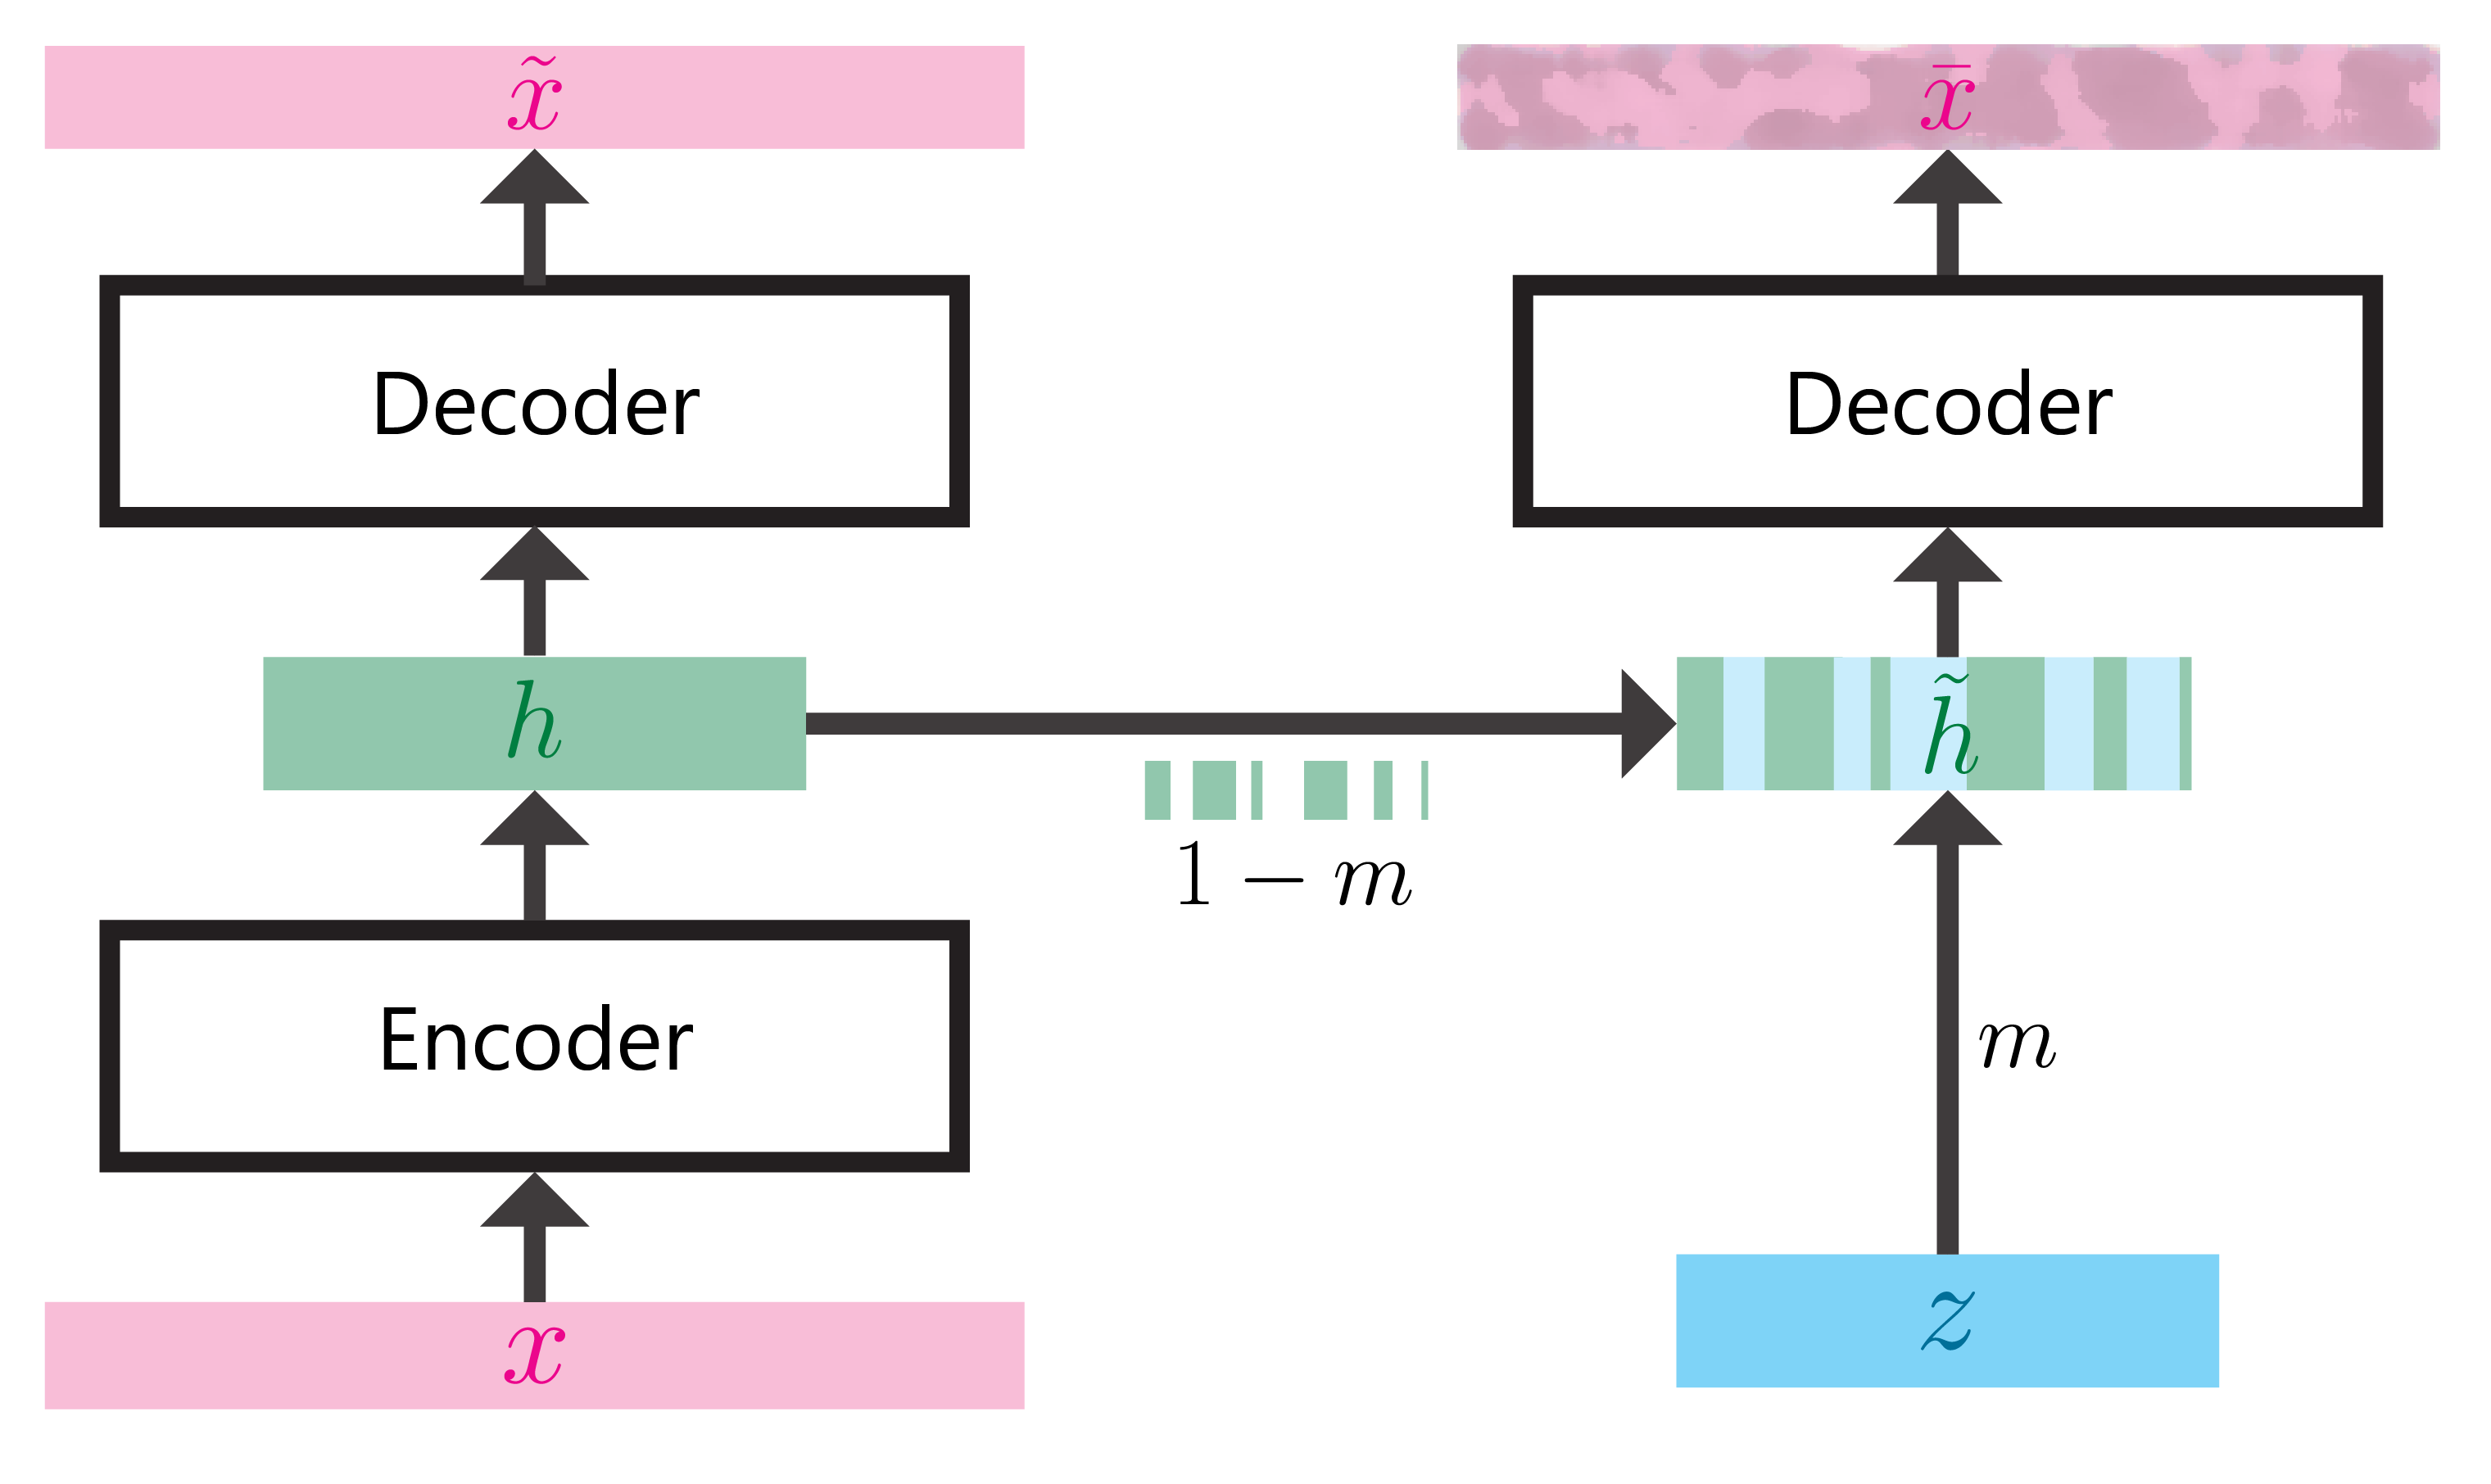
\includegraphics[width=1\columnwidth]{assets/transitional}
\end{tcolorbox}
\normalsize
\end{figure}%
            %
            
            \Gls{ssl} is commonly used to augment the minority class in imbalanced datasets, with techniques such as \gls{st} and \gls{ct}. \citeauthor{yang2018unpaired} improve on both by incorporating a \gls{gan} in the procedure \cite{yang2018unpaired}. The \gls{gan} is first trained on the labelled set and used to re-balance it. A prediction task with a classifier ensemble is then executed and the data points with highest prediction confidence are labelled. The process is iterated until labelling expansion ceases. As a final step, the \gls{gan} is trained on the expanded labelled set to generate an equal amount of augmentation data. The authors obtained improved performance in a number of classification tasks and multiple tabular datasets.
    
    \subsubsection{Domain translation}
    
        To address the heterogeneity of healthcare data originating from different sources, \citeauthor{Yoon2018-radial} combines the concepts of cycle-consistent domain translation from \gls{cycle-gan} \cite{Zhu_2017} and  multi-domain translation from Star-GAN \cite{choi2017stargan} to build \gls{radialgan} to translate heterogeneous patient information from different hospitals, correcting features and distribution mismatches \cite{Yoon2018-radial}. One encoder-decoder pair per data endpoint that are trained to map records to and from a shared latent representation for their respective endpoint. 
    
    \subsubsection{Individualized treatment effects}
    
        The task of estimating \glspl{ite} is an ongoing problem. \glspl{ite} refer to the response of a patient to a certain treatment given a set of characterizing features. The problem is that counterfactual outcomes are never observed or treatment selection is highly biased \cite{Yoon2018-ite, mcdermott2018semi, walsh2020generating}. In \gls{ganite} \citeauthor{Yoon2018-ite} propose a solution by using a pair of \glspl{gan}: one for counterfactual imputation and another for \gls{ite} estimation \cite{Yoon2018-ite}. The former captures the uncertainty in unobserved outcomes by generating a variety of counterfactuals. The output is fed to the latter, which estimates treatment effects and provides confidence intervals.\par
    
        \citeauthor{mcdermott2018semi} developed \gls{cwr-gan} to leverage large amounts of unpaired pre/post-treatment time-series in \gls{icu} data for the estimation of \glspl{ite} on physiological time-series \cite{mcdermott2018semi}. \gls{cwr-gan} is a joint regression-adversarial  \gls{ssl} approach inspired by \gls{cycle-gan}. The algorithm has the ability to learn from unpaired samples, with very few paired samples, to reversibly translate the pre/post-treatment physiological series.\par 
    
        \citeauthor{chu2019treatment} address the problem of data scarcity by designing \gls{adtep}. The algorithm can harness the large volume of \gls{ehr} data formed by triples of non-task specific patient features, treatment interventions and treatment outcomes \cite{chu2019treatment}. \gls{adtep} learns representation and discriminatory features of the patient, and treatment data by training an \gls{ae} for each pair of features. In addition to \gls{ae} reconstruction loss, a second discriminator is tasked with identifying fake treatment feature reconstructions. Finally, a fourth loss metric is calculated by feeding the concatenated latent representations of both \glspl{ae} to a \gls{lr} model aimed at predicting the treatment outcome \cite{chu2019treatment}.\par
    
        Like \citeauthor{esteban2017real}, \citeauthor{Wang_2019} demonstrated an algorithm to generate a time series of patient states and medication dosages pairs using \gls{lstm}. In contrast to \gls{rgan} and \gls{rcgan}, in \gls{sc-gan}, patients state at the current time-step informs the concurrent medication dosage, which in turn affects the patient state in the upcoming time-step \cite{Wang_2019}. \gls{sc-gan} overcame a number of baselines on both statistical and utility metrics.
    
    \subsubsection{Data imputation and augmentation}
    
        \gls{gan} are naturally suited for data imputation, and can mitigate missingness. Statistical models developed for the multiple imputation problem increase quadratically in complexity with the number of features, while the expressiveness of deep neural networks can efficiently model all features with missing values simultaneously.\par
        In that regard, \citeauthor{yoon2018imputation} adapted the standard \gls{gan} to perform imputation on real-valued features \gls{mar} in tabular datasets \cite{yoon2018imputation}. In \gls{gain}, the discriminator must classify individual variables as real or fake (imputed), as opposed to the whole ensemble. Additional input, or hint, containing the probability of each component being real or imputed is fed to the discriminator to resolve the multiplicity of optimal distributions that the generator could reproduce. The model performs considerably better than five state-of-the-art benchmarks. \gls{gain} was later adapted by \citeauthor{Yang_2019_impute_ehr} to also handle categorical features using fuzzy binary encoding, the same technique employed in \gls{healthgan}. In parallel, \citeauthor{Camino2019} apply the same \gls{vs} technique they used fir \gls{medgan} to adapt \gls{gain} and run a benchmark against different types of \gls{vae}.\par
    
        The distribution estimated by a generator can compensate for lack of diversity in a real sample, essentially filling in the blanks in a manner comparable to data imputation. In such cases, data sampled from this distribution has the potential to help improve generalization in training predictive models. As an example, we mentioned generating unobserved counterfactual outcomes \cite{yoon2018imputation}, and generating neighboring samples to help generalization in predictors \cite{Che_2017}.\par 
        The adversarially trained \gls{rmb} developed by \citeauthor{Fisher2019} enabled them to simulate individualized patient trajectories based on their base state characteristics. Due to the stochastic nature of the algorithm, generating a large number of trajectories for a single patient can provide new insights on the influence of starting conditions on disease progression or quantify risk \cite{Fisher2019}.
        
    \subsection{Model validation and data evaluation}
    
        To asses the solution to a generative modelling problem, it is necessary to validate the model, and to verify its output. \gls{gan} aim to approximate a data distribution $P$, using a parameterized model distribution $Q$ \cite{Borji2018-fy}. Thus, in evaluating the model, the goal is to validate that the learning process has led to a sufficiently close approximation. What this means in practice is hard to define. The concept of "realism" finds more natural application to images of text, but becomes ambiguous when faced with the complexity of health data.\par
        
        \citeauthor{walsh2020generating} employ the term "statistical indistinguishability" and define it as the inability of a classification algorithm to differentiate real from synthetic samples \cite{walsh2020generating}. The terms covers almost all evaluation methods employed in the publications, which can be divided into two broad categories: those aimed at evaluating the statistical properties of the data directly, and those aimed at doing so indirectly by quantifying the work that can be done with the data. There are, nonetheless a few attempts of a qualitative nature, more in line with the concept of realism. 

        \subsubsection{Qualitative evaluation}
        
            Visual inspection of projections of the \gls{sd} is a common theme, serving mostly as a basic sanity check, but occasionally presented as evidence. The formal qualitative evaluation approaches found in the literature are mainly Preference Judgement, Discrimination Tasks or Clinician Evaluation and are generally carried out by medical professionals (Borji 2018).
                \begin{itemize}
                    \item \textbf{Preference judgment} The task is choosing the most realistic of two data points in pairs of one real and one synthetic \cite{Choi2017-nt}.
                    \item \textbf{Discrimination Tasks} Data points are shown one by one and must be classified as real or synthetic \cite{Beaulieu-Jones2019-ct}.
                    \item \textbf{Clinician Evaluation} Rather than classifying the data points, they must be rated for realism according to a predefined numerical scale. \cite{Beaulieu-Jones2019-ct}. Significance is determined with a statistical test such as Mann-Whitney.
                    \item \textbf{Visualized embeding} The real and synthetic data samples are plotted on a graph or projected into an embeding such as \gls{t-sne} or PCA and compared visually. \cite{cui2019conan, yu2019rare, zhu_2020, yale2019ESANN, Yang_2019_ehr,Beaulieu-Jones2019-ct, tanti2019, dash2019synthetic}.
                    \item \textbf{Feature analysis} In certain fields, the data can be projected to representations that highlight patterns or properties that can be easily visually assessed. While this does not provide conclusive evidence of data realism, it can help get a better understanding of model behaviour during training. As an example, typical and easily distinguishable patterns in EEG and ECG bio-signals. \cite{Harada2019}
                \end{itemize}
    
        In general, qualitative evaluation methods based on visual inspection are weak indicators of data quality. At the dataset or sample level, quantitative metrics provide more convincing evidence of data quality (Borji 2018).
        
        \subsubsection{Quantitative evaluation}
        
            Quantitative evaluation metrics can be categorized into three loosely defined groups: comparing the distributions of real and synthetic data as a whole, assessing the marginal and conditional distributions of features, and evaluating the quality of the data indirectly by quantifying the amount of work that can be done with the data, referred to as utility.
            
            \begin{itemize}
                \item \textbf{Dataset distributions}
                A summary of metrics is presented in Tab. \ref{tab:3:distributions}.
                \item \textbf{Feature Distributions}
                If the model has learned a realistic representation of the real data it should produce \gls{sd} that possesses the same quantity and type of information content. Authors attempt by various metrics to determine if the statistical properties of the \gls{sd} agree with those of the real data. These metrics are presented in Table \ref{tab:3:statistics}. Although statistical similarity provides strong support for the behavior of the learning process, it is not necessarily informative about their validity. They are often ambiguous and can be found to be misleading upon further investigation. Given the complexity of health data, low level relations are unlikely to paint a full picture. Authors often state that no single metric taken on its own was sufficient, and that a combination of them allowed deeper understanding of the data.
                \item \textbf{Data utility}
                 Utility-based metrics, presented in Table \ref{tab:3:augmentation}, often provide a more convincing indicator of data realism. On the other hand, they mostly lack the interpretability of statistical metrics. We took the liberty of placing these into one of two categories: tasks mostly defined only for evaluation (Ad hoc utility metrics) or tasks based on real-world applications (Application utility metrics). Note that this distinction is not based on a rigorous definition, but serves to facilitate comparison.
                \item \textbf{Analytical} The analytical methods were mainly employed for evaluation, but can also provide a better understanding of the and its behavior.
                \begin{itemize}
                    \item \textsl{Feature Importance} The important features (\gls{rf}) and model coefficients (\gls{lr}, \gls{svm}) of predictors. \cite{esteban2017real,Xu2019-ay,Yoon2020-anon,chin2019generation, Beaulieu-Jones2019-ct}.
                    \item \textsl{Ablation study}  The performance of the model is compared against impaired version. This helps determining if the novel component of the algorithm contributes significantly to performance \cite{cui2019conan, Che_2017, mcdermott2018semi, Yoon2018-radial, chincheong2020generation}.
                \end{itemize}
            \end{itemize}
            
                 \begin{table}[H]         
 \footnotesize  
 \setlength{\extrarowheight}{0.5em}
 \caption{Metrics employed to validate trained models based on the comparison of distributions.\label{tab:3:distributions}}              
    \begin{tabular}{@{} p{0.2\textwidth} p{0.8\textwidth} @{}}\toprule                          
    Metric & Description \\ \midrule                                  
    
    \gls{kld} 
    & Non-symmetric measure of difference between two \glspl{pd}, related to relative entropy. Given a feature $X$, $p(x)$ and $q(x)$ the \gls{pd} of the real and synthetic data respectively, the \gls{kld} of $q(x)$ from $p(x)$ is the amount of information lost when $q(x)$ is trained to estimate $p(x)$ \cite{klb2008, Goncalves2020}. \\       
    
    \gls{rdp} 
    & Alternative measure of divergence, which includes \gls{kld} as a special case. The \gls{rdp} includes a parameter $\alpha$ that gives it an extra degree of freedom, becoming equivalent to the Shannon-Jensen divergence when $\alpha \longrightarrow 1$. It showed a number of advantages when compared to the original \gls{gan} loss function, and removed the need for gradient penalty \cite{VanBalveren2018, tanti2019}\\ 
    
    Jaccard similarity & Measure of similarity and diversity defined on sets as the size of the intersection over the size of the union \cite{ozyigit2020generation, Yang_2019_ehr, Wikipediacontributors}.\\

    2-sample test (2-ST) 
    & Statistical test of the null hypotheses the real and \gls{sd} samples came from the same distribution. and synthetic, originate from the same distribution through the use of a statistical test such as \gls{ks} or \gls{mmd}.\cite{Fisher2019,baowaly_2019_IEEE,baowaly_2019_jamia,esteban2017real}\\     
    
    Distribution of Reconstruction Error 
    & Compares the distributions of reconstruction error for the \gls{sd} and the training set versus the \gls{sd} and a held out testing set. Calculated according to the Nearest-neighbor metric or other measures of distance. A significant difference would indicate over-fitting and can evaluated with a statistical test, such as \gls{ks}. \cite{esteban2017real}\\
    
    Latent space projections 
    & Real and synthetic samples are projected back into the latent space, or encoded with a \gls{beta-vae}, comparing the dimensional mean of the variance or the distance between mode peaks \cite{Zhang2020}. See Section \ref{sec:latent-space} for examples of how the latent space encoding can interpreted. \\
    
    \glspl{dsm} 
    & Comparison of the \gls{pd} with \glspl{dsm}. For instance the Quantile-Quantile (Q-Q) plot for point-processes \cite{Xiao2017-lh}. See Section \ref{sec:evaluation-cqm} for a notion of how \glspl{dsm} could apply to \gls{ehr} data.\\                              
    Classifier accuracy &  
    Accuracy of a classifier trained to discriminate real from synthetic units. Predictor accuracy around 0.5 would indicate indistinguishability. \cite{Fisher2019,walsh2020generating}\\       
    
    \bottomrule                      
    \end{tabular}         
\end{table}
                \begin{table}[H]
        \footnotesize
        \setlength{\extrarowheight}{0.5em}
        \caption{Metrics based on evaluating the statistical properties of the synthetic data distribution. \label{tab:3:statistics}}
        \begin{tabularx}{\textwidth}{@{} p{0.3\textwidth} X @{}}\toprule
            Metric & Description\\ \midrule
            
            Dimensions-wise distribution & 
            The real and synthetic data are compared feature-wise according to a variety of methods For example, the Bernoulli success probability for binary features, or the Student T-test for continuous variables, and Pearson Chi-square test for binary variables is used to determine statistical significance \cite{Beaulieu-Jones2019-ct,Choi2017-nt,chin2019generation,yan2020generating,baowaly_2019_IEEE,baowaly_2019_jamia,ozyigit2020generation,tanti2019, Yoon2020-anon, tanti2019, Fisher2019, Che_2017, Wang_2019, yale2019ESANN, chincheong2020generation, ozyigit2020generation}.\\
            
            Inter-dimensional correlation & 
            Dimension-wise Pearson coefficient correlation matrices for both real and synthetic data \cite{Beaulieu-Jones2019-ct, Goncalves2020, torfi2019generating,Frid_Adar_2018,ozyigit2020generation, Yang_2019_ehr, Yoon2020-anon, zhu_2020, Yoon2020-anon, walsh2020generating, yale2019ESANN, ozyigit2020generation, Dash, Bae2020}.\\
           
            Cross-type Conditional Distribution & 
            Correlations between categorical and continuous features, comparing the mean and standard deviation of each conditional distribution \cite{yan2020generating}.\\
            
            Time-lagged correlations & 
            Measures the correlation between features over time intervals.
            \cite{Fisher2019,walsh2020generating}.\\
            
            Pairwise mutual information & 
            Checks for the presence multivariate relationships pair-wise for each feature, as a measure of mutual dependence \cite{Rankin2020}. Quantifies the amount of information obtained about a feature from observing another.\\
            
            First-order proximity metric & 
            Defined over graphs, captures the direct neighbor relationships of vertices. \citeauthor{Zhang2020} applied to graphs built from the co-occurrence of medical codes and compared the results between real and synthetic data \cite{Zhang2020}.\\
            
            Log-cluster metric & 
            Clustering is applied to the real and synthetic data combined. The metric is calculated from the number of real and synthetic samples that fall in the same clusters \cite{Goncalves2020}.\\
            
            Support coverage metric & 
            Measures how much of the variables support in the real data is covered in the synthetic data. Support is defined as the percentage of values found in the synthetic data, while coverage is the reverse operation. The metric is calculated as the average of the ratios over all features. Penalizes less frequent categories that are underrepresented \cite{Goncalves2020}.\\
 
            Proportion of valid samples & 
            Defined by \citeauthor{Yang_2019_ehr} as a requirement for records to contain both disease and medication instances. \cite{Yang_2019_ehr}.\\
            
            \gls{pca} Distributional Wassertein distance 
            & The Wassertein distance is calculated over k-dimensional \gls{pca} projections of the real and synthetic data \cite{tanti2019}.\\
            
            \bottomrule
        \end{tabularx}
    \end{table}
                \begin{table}[H]
        \footnotesize
         \setlength{\extrarowheight}{0.5em}
        \caption{Metrics based on evaluating the utility of the synthetic data on practical tasks.}\label{tab:3:augmentation}
        
        \begin{tabularx}{\textwidth}{@{} p{0.2\textwidth} X @{}} \toprule
        Metric & Description \\ \midrule
        
        \multicolumn{2}{c}{\textbf{Data utility metrics}}\\ \midrule
        
        \gls{dwp} & Each variable is in turn chosen as the prediction target label and the remaining as features. Two predictors are trained to predict the label, one from the synthetic data and another from a portion of the real data. Their performance is compared on the left out real data \cite{Choi2017-nt,Camino2018-re,Goncalves2020,yan2020generating, tanti2019, baowaly_2019_IEEE}.\\
        
        \gls{arm} & \gls{arm} aims to the discovery of relationships among a large set of variables, commonly occurring variable-value pairs \cite{Agrawal1993}. The rules obtained from the real and synthetic data are compared \cite{baowaly_2019_IEEE,baowaly_2019_jamia,BaeAnomiGAN2020,yan2020generating}.\\
        
        Training utility & Performance of predictors trained on the synthetic data, often in comparison with the real data or data generated with \gls{dp} \cite{BaeAnomiGAN2020}.\\
        
        \gls{trts} & Accuracy on real data of some form of predictor trained on synthetic data \cite{Beaulieu-Jones2019-ct, Rankin2020, Yoon2020-anon}. \\ 
        
        \gls{tstr} & Accuracy on synthetic data of some form of predictor trained on real data   \cite{BaeAnomiGAN2020, Yoon2020-anon, Jordon2019}.\\
        
        Discriminator & A predictor is trained to discriminate synthetic from real sample. An accuracy value of 0.5 would indicate that they are indistinguishable \cite{Fisher2019, walsh2020generating, yale:hal-02160496}.\\ 
        
        Siamese discriminator & A pair of identical \gls{ffn} each receive either a real sample or a synthetic sample. Their output is passed to a third network which outputs a measure of similarity \cite{torfi2019generating}.\\\midrule

        \multicolumn{2}{c}{\textbf{Applied utility metrics}}\\ \midrule
        
        Data augmentation & A predictor is trained on a combination dataset of real and synthetic data or real data with missing values imputed and performance is compared with the same predictor trained on real data alone \cite{Yoon2020-anon, Yang_2019_cdss, Yang_2019_ehr}.\\
        
        Model augmentation & The trained generative model is incorporated into a predictor's activation function by generating an ensemble of proximate data points for each instance, thereby improving generalization \cite{Che_2017}.\\
        
        Accuracy & The prediction performance of the model is compared against benchmarks of the same type on real data \cite{cui2019conan, Yoon2018-ite, Che_2017, yu2019rare, zhu_2020, baowaly_2019_IEEE, Wang_2019, walsh2020generating, yoon2018imputation, mcdermott2018semi, Yang_2019_ehr, Yoon2018-radial, Xu2019-ay, Beaulieu-Jones2019-ct, BaeAnomiGAN2020}. Models trained to make forward predictions from past observations or from real data transformed with a known function can simply be evaluated for accuracy. For example, the \gls{rmse} on time-series \cite{Xiao2018-aj,mcdermott2018semi,yoon2018imputation,Yang_2019_cdss, zhu_2020}.\\
        
        \bottomrule
        
        \end{tabularx}
\end{table}

    \subsection{Alternative evaluation}
        In their publications, \citeauthor{Yale_2020} propose refreshing approaches to evaluating the utility of \gls{sd}. For example, they organized a hack-a-thon type challenge involving the data. During the event, students were tasked with creating classifiers, while provided only with \gls{sd} \cite{Yale_2020}. They were then scored on the accuracy of their model on real data.\par
        In more rigorous initiatives, they attempted (successfully) to recreate the experiments published in medical papers based on the MIMIC dataset using only data generated from their model \gls{healthgan}. In a subsequent version of their article, the authors evaluate the performance of their model against traditional privacy preservation methods by using the trained discriminator component of \gls{healthgan} to discriminate real from synthetic samples.
        
    \subsection{Privacy}
        Some authors conducted a privacy risk assessment to evaluate the risk of reidentification. The empirical analyses were based on the definitions of \gls{mi}, \gls{ad}  \cite{Choi2017-nt,Goncalves2020,yan2020generating,chen2019ganleaks, chincheong2020generation} and the \gls{rr} \cite{Zhang2020}. Cosine similarities between pairs of samples was also used \cite{torfi2019generating}. Most studies report low success rates for these types of attacks, and little effect from the sample size, although \citeauthor{chen2019ganleaks} note that sample sizes under 10k lead to higher risk. \citeauthor{Goncalves2020} evaluated \gls{mc-medgan} against multiple non-adversarial generative models in a variety of privacy compromising attacks, including \gls{ad}, obtaining inconsistent results for \gls{mc-medgan} \cite{Goncalves2020}. While this is not mentioned by the authors, multiple results reported in the publication point to the fact that the \gls{gan} was not properly trained or suffered mode-collapse.In black-box and white-box type attacks, including the LOGAN \cite{hayes2017logan} method, \gls{medgan} performed considerably better than \gls{wgan-gp} \cite{chen2019ganleaks}, the algorithm which served as basis for improvements to \gls{medgan} in publications discussed in Section \ref{subsubsec:categorical}. Overall, the author notes that releasing the full model poses a high risk of privacy breaches and that smaller training sets (under 10k) also lead to a higher risk. \par
        \subsubsection{The status of fully synthetic data in regards to current privacy regulations}
        
            It seems intuitively possible that the artificial nature of \gls{sd} essentially prevents associations with real patients, however the question is never directly addressed in the publications. An extensive Stanford Technological Review legal analysis of \gls{sd} concluded that laws and regulations should not treat \gls{sd} indiscriminately from traditional privacy preservation methods \cite{bellovin2019privacy}. They state that current privacy statutes either outweigh or downplay the potential for \gls{sd} to leak secrets by implicitly including it as the equivalent of anonymization. 
            
        \subsubsection{Traditional privacy}
        
            Numerous attempts at applying traditional privacy guarantees, such as deferentially-private stochastic gradient descent can also be found in other fields, as well as in healthcare \cite{Beaulieu-Jones2019-ct, esteban2017real,chincheong2020generation, BaeAnomiGAN2020}. By limiting the gradient amplitude at each step and adding random noise, AC-GAN could produce useful data with $\epsilon=3.5$ and $\delta<10^{-5}$ according to the definition of differential privacy. \par 
        
        \subsubsection{Moving forward safely}
        
            Some have put forward the notion that preventing over-fitting and preserving privacy may not be conflicting goals \cite{Wu2019-ui,Mukherjee2019-vu,Zhu2020-oj}. Letting go of the negative connotation, we can explore the benefits such as improving generalization, stabilizing learning and building fairer models \cite{Zhu2020-oj} and the use of \glspl{gan} to optimize the trade-off \cite{Chen2019-mh}.\par
            
            \begin{itemize}
                \item \citeauthor{BaeAnomiGAN2020} ensure privacy with a probabilistic scheme that ensure indistinguishably, but also maximizes utility. Specifically, a multiplicative perturbation by random orthogonal matrices with input entries of $k x m$ medical records and a second second discriminator in the form of a pre-trained predictor \cite{BaeAnomiGAN2020}.
                \item In privGAN \cite{Mukherjee2019-vu}, an adversary is introduced, forcing the generator to produce samples that minimize the risk of \gls{mi} attacks, in addition to cheating the discriminator. The combination of both goals has the explicit effect of preventing over-fitting, and their algorithm produces samples of similar quality to non-private \gls{gan}.
            \end{itemize}
           \subsubsection{Alternative views of privacy}
            The discordance between the theoretical concepts of DP, which are  based ultimately on infinite samples, and the often insufficient data on which the probability of disclosure is calculated remains deficient. Therefore, Yoon et al. have postulated an intriguing alternative view of privacy \cite{Yoon2020-anon}. They propose to emphasize measuring identifiability of finite patient data, rather than the probabilistic disclosure loss of DP based on unrealistic premises. Simplistically, they define identifiability as the minimum closest distance between any pair of synthetic and real samples. This echoes the concept of t-closeness \cite{Li2010-qq}. In their implementation, the generator receives both the usual random seed and a real sample as input. This has the effect of mitigating mode collapse, but also of raises the risk of reproducing the real samples. The discriminator is equipped with an additional loss metric based on a measure of similarity between the original sample and the generated one, thus ensuring a tune-able threshold of identifiability. Their results on a number of previously discussed evaluation metrics are encouraging.\par
            
            In a similar approach, \citeauthor{Yale_2020} broke away from the theoretical guarantees of traditional methods with a measure native to \glspl{gan}. Their proposal is a metric quantifying the loss of privacy, a concept more aligned with the objective of \gls{gan} to minimize the loss of data utility \cite{yale:hal-02160496,p2019}. They point out, the advantage of concrete measurable values of loss in utility and privacy when making the decision of releasing sensitive data. Briefly, the Nearest Neighbor Adversarial Accuracy measures the loss in privacy based on the difference between two nearest neighbor metrics. The  first component is the proportion of synthetic samples that are closer to any real sample than any pair of real samples. The second component is the reverse operation. In a subsequent paper, \gls{healthgan} evaluated against traditional privacy preservation methods with a variant of the IA based on the nearest neighbor metric. \gls{healthgan} performs considerably better than all other methods, while still maintaining utility on a prediction task.


       



